\chapter{Background}

\begin{displayquote}
``Amateur radio is a popular technical hobby and volunteer public service that uses designated radio frequencies for non-commercial exchange of messages, wireless experimentation, self-training, and emergency communications.
Amateur Radio is the only hobby governed by international treaty.'' \cite{def_amateur_radio}
\end{displayquote}

Often for operators it would be more convenient to control their radios remotely. This is sometimes known more commonly as a ``remote shack''. In this scenario as much remote control as possible is desired. This is often achieved using existing commercial or home made solutions that rely on simply repeating control signals. For example the RRC 1258Mk is a product designed to do this. It is priced at \$708\cite{RRC_1258Mk} is perhaps prohibitively expensive as it is two times the price of the radio. Instead it would be preferable to understand and/or emulate these signals. The end result is that the radio gains \gls{cat}\cite{CAT} features.

Remote shacks are geographically positioned for their prime transceiving properties, for example on the top of a hill so the signal is less affected by the geometry of the surrounding area. They are often limited in their connectivity to utilities, such as power or Internet connection. This is especially in extremely remote areas where communication is sometimes done over telephone networks.

An ideal scenario for these kind of users is where all functions can be controlled from the radio remotely, using as little data traffic as possible. This use-case also extends to users that prefer to use a PC to control their radios. This may be for more features, better user experience (given by software), or possibly for accessibility reasons (i.e where reading the screen or using the small dials would be a problem for the operator).

\begin{figure}[H]
    \centering
    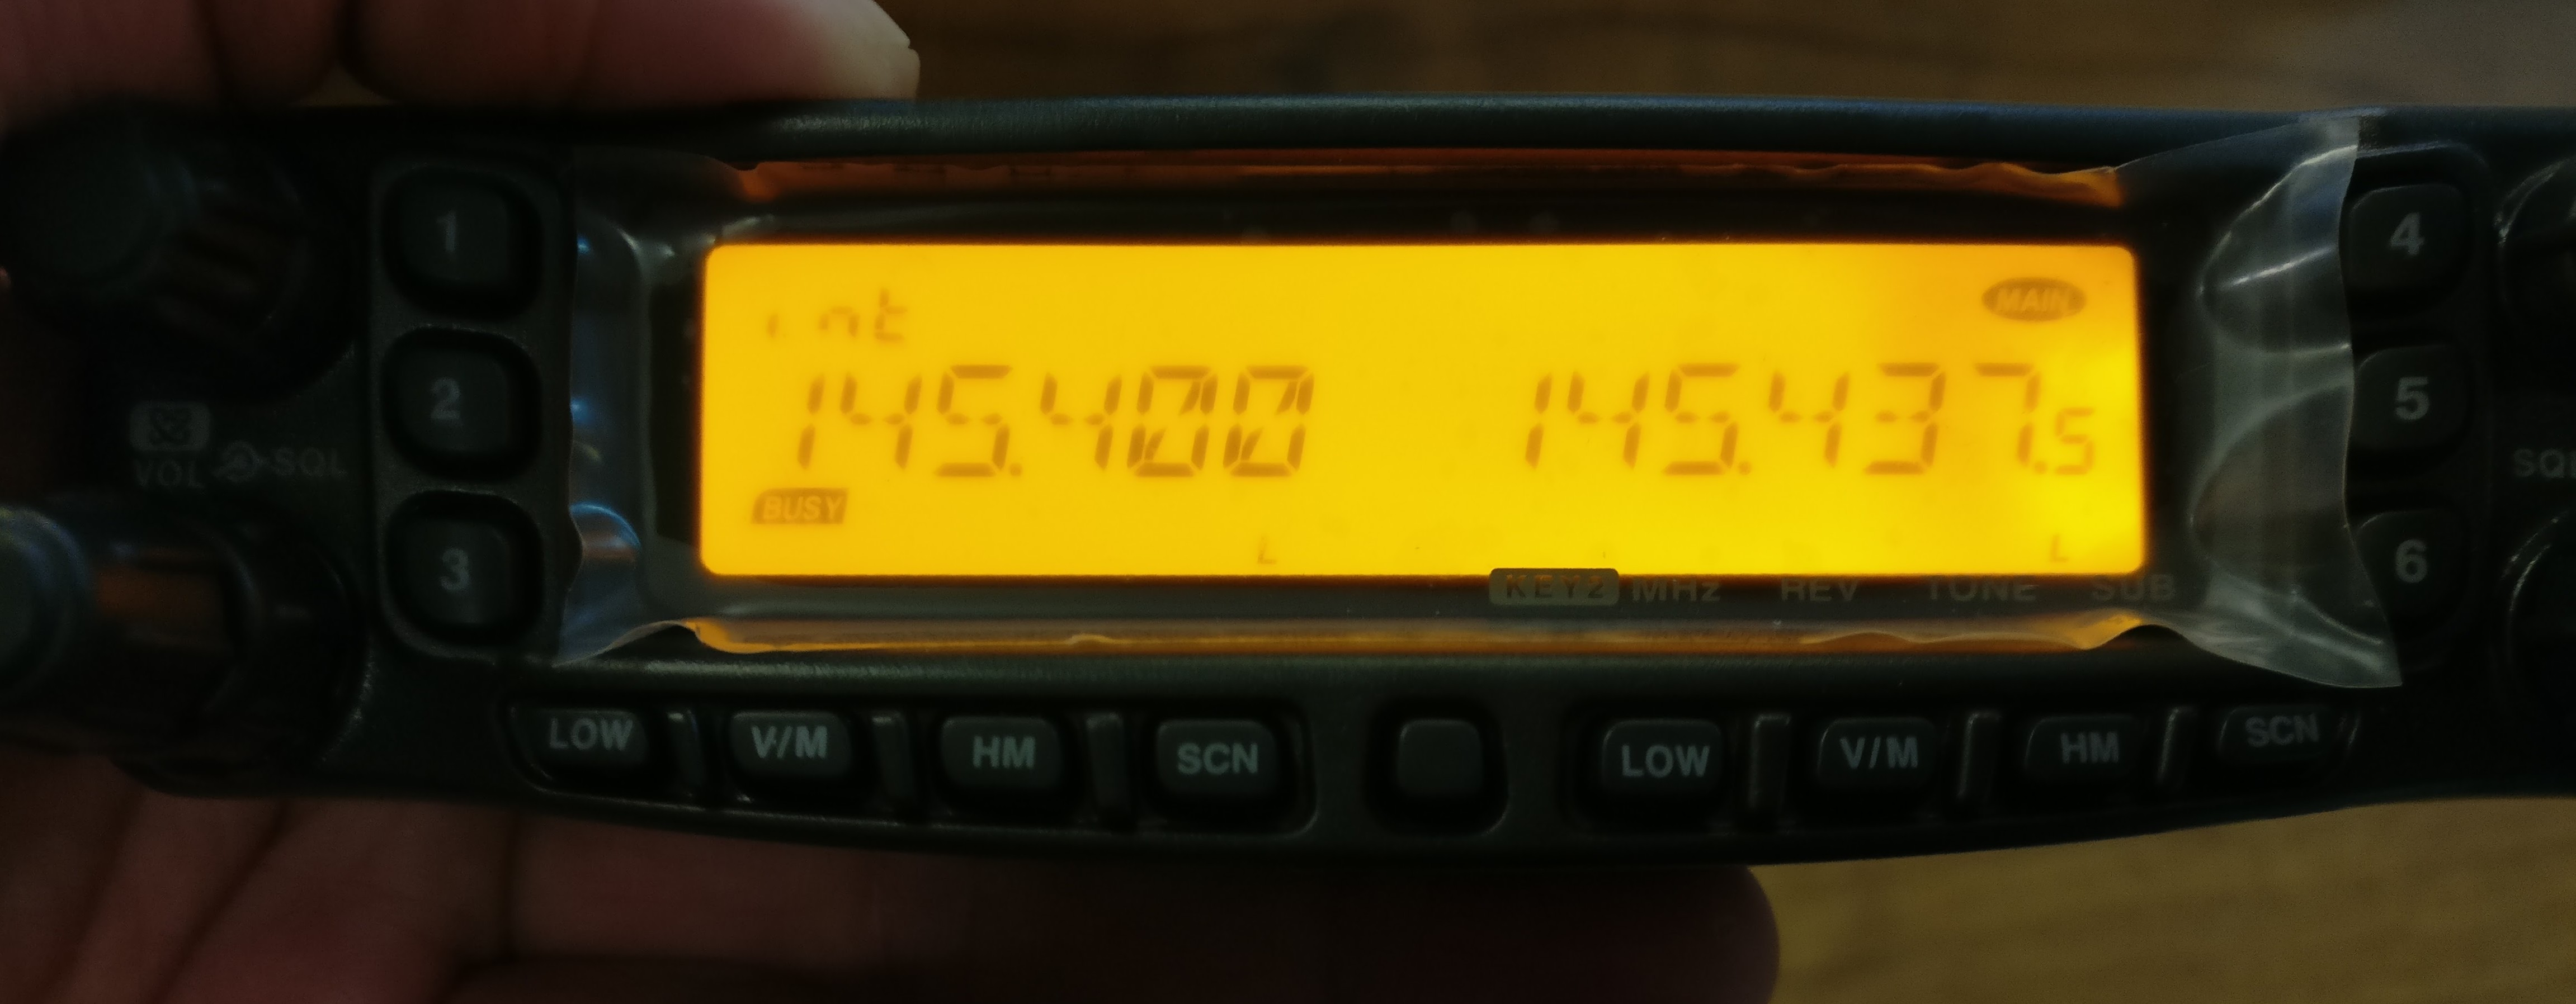
\includegraphics{img/radio_head.jpg}
    \caption[Picture of RT-8900r radio]{A picture of the face of the RT-8900r radio.}
    \label{fig:radio_head}
\end{figure}

The \gls{8900} (Seen in figure~\ref{fig:radio_head}) is a popular, budget amateur radio, it is marketed for mobile applications such as being mounted on a car dashboard. This is achieved using a control surface (hereby referred to as the head) that is detachable from the rest of the body of the radio. This allows the body to be mounted in a more practical location by running a control cable between the two.

The main goal of this project is to allow the functions of the radio to be available from a computer. This will be achieved by adapting the \gls{8900} to have \gls{cat} features. Radios that come with this feature typically have a serial port or some kind. My project relies on the assumption that it is possible that the control line can be intercepted and emulated by a computer. This means that functionality could be added in a similar way to radios that advertise the C.A.T feature. This must be achieved cost effectively and in a simple way for the user to create and setup by themselves. Any designs and software will then be released under the Gnu Public Licence (v3) for the benefit of the community.

I originally chose the project as it seemed like a good way to learn several topics that interested me. Primarily the topics of reverse engineering and driver authoring. While these elements existed in my project they where not as prominent as I had first an anticipated (although I still enjoyed the experience regardless). 